\documentclass[../poliXuniversity_hospital_(USP)_report.tex]{subfiles}
\graphicspath{ {images/}{../images/} } 

\begin{document}
\chapter{Modulos Embarcados}

\begin{figure}[h]
\centering
    \caption{Módulos Embarcados - Robô Hospitalar (V2)}
    \centering % para centralizarmos a figura
    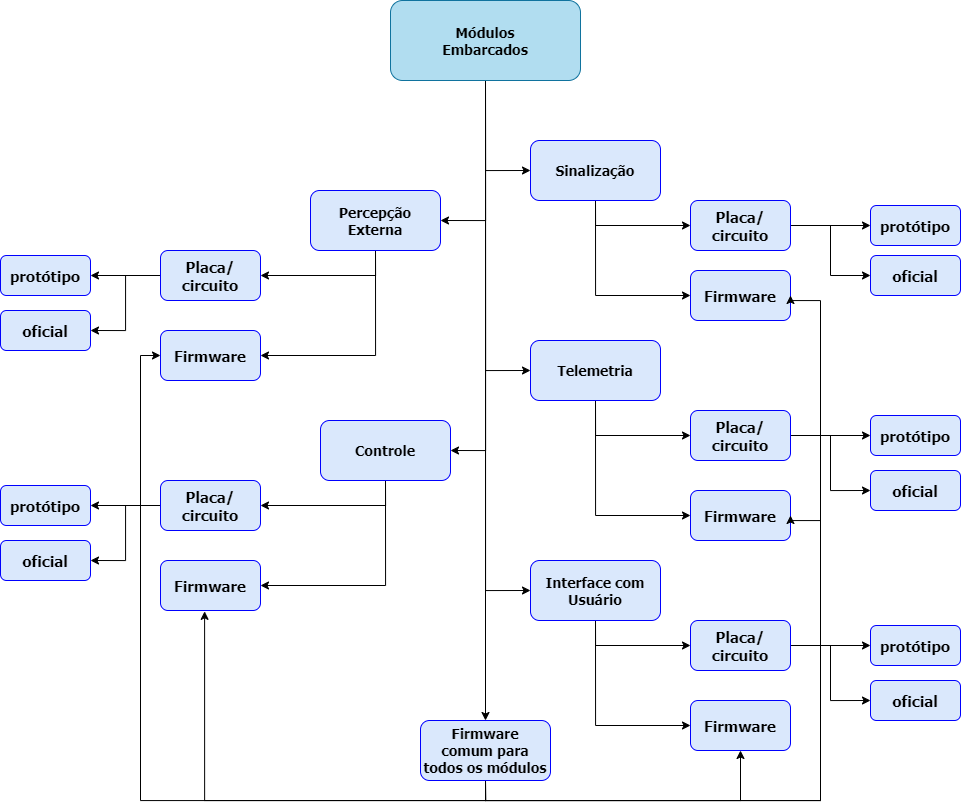
\includegraphics[width=15cm]{modulos_embarcados.png}
    \caption*{Fonte: Elaborada pelo autor}
    \label{figura:1° Versão Robô Hospitalar}
\end{figure}

 Os módulos embarcados, ou eletrônicos do Robô Hospitalar (V2) foram divididos por função específica, dessa forma, cada módulo tem um pequeno trabalho diante o robô todo. Dentre esses cinco módulos, um deles, como se fosse um líder ou mestre, tem função de receber as informações dos outros módulos e se comunicar com o computador embarcado no robô, a Jetson Nano \cite{jetson21}, Cada um desses módulos recebeu um nome específico, sendo eles: Sinalização, Telemetria, Percepção Externa, Interface com Usuário e Controle.

Nos primórdios, ela foi feita para facilitar a manutenção do robô e troca eventual de alguns dos módulos. Por mais que essa organização exige mais microcontroladores e aumenta a complexidade da confecção dos códigos embarcados, ainda se mostra bem interesse em termos de manutenção.

Por mais que cada módulo tenha sua característica que o torne único, há diversos parâmetros e componentes que todos os módulos tiveram ou têm em comum entre todos.  Dentre eles, tantos nos protótipos e versões oficiais, destaca-se o microcontrolador, as dimensões da placa, encapsulamento e protocolos de comunicação.

%------------------------------------------
\begin{wrapfigure}{r}{5.5cm}
\caption{Microcontrolador ESP32}\label{wrap-fig:1}
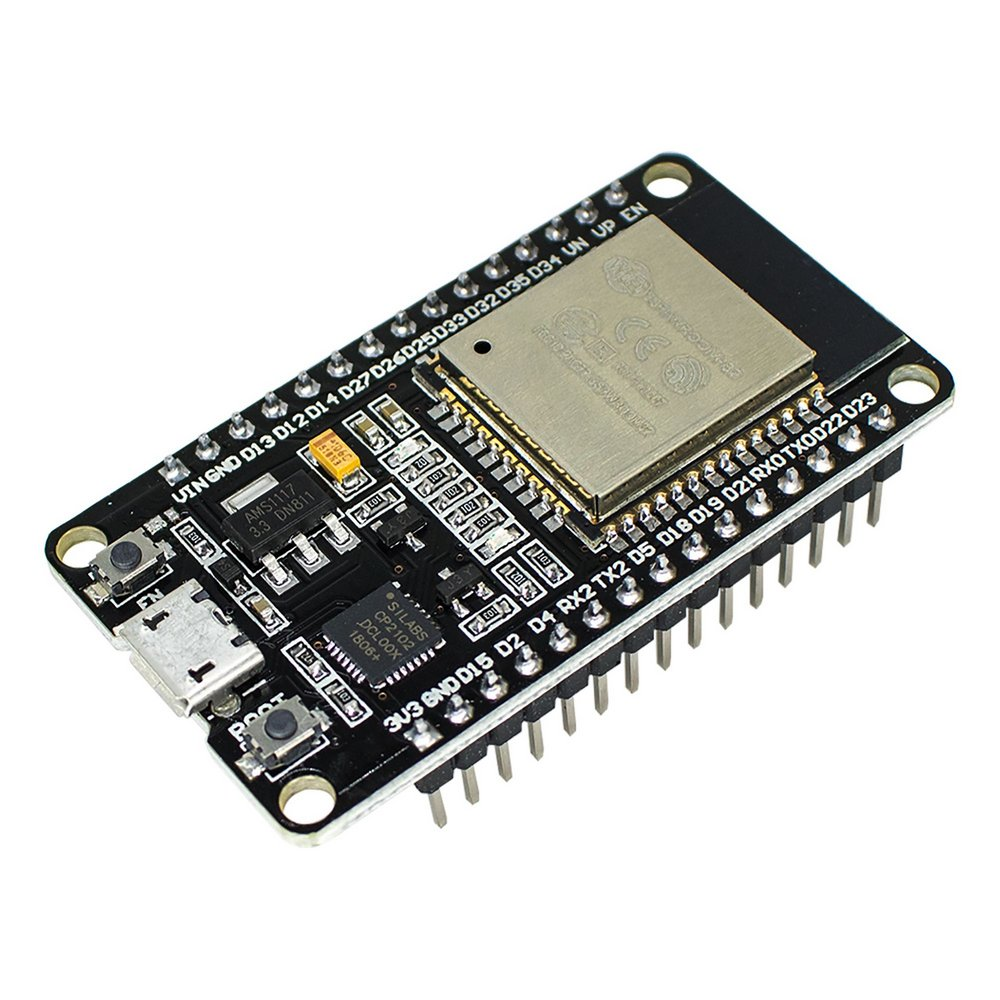
\includegraphics[width=7cm]{esp32_doidkit_v1.jpg}
\caption*{Fonte: Foto disponibilizada por saravati}\label{wrap-fig:1}
\end{wrapfigure} 
%------------------------------------------

O microcontrolador padrão escolhido para todos os módulos foi ESP32 \cite{esp32}, que é dentre os mais famosos, como Arduino \cite{arduino}, o que apresenta a maior capacidade de  processamento e ainda é mais barato que os convencionais \cite{esp32_better}, além de já ter um módulo bluetooth embutido. Por conta desses motivos que adotamos o ESP32 como micro controlador padrão.

Para realizar a comunicação entre os ESP32 \cite{esp32}, a princípio, seria utilizado somente o protocolo I2C \cite{i2c} para haver a troca de mensagem entre os módulos. Todas as placas fresadas, ou seja, que ainda são protótipos, só tinham esse protocolo de comunicação. No entanto, por conta da instabilidade do protocolo I2C, foi adicionado conexões SPI \cite{spi}, que é muito mais rápido que o convencional e ainda tem mais instabilidade no esquemático.

Além disso, todas as placas têm a sua dimensão constante. Todos os protótipos tinham, dimensões de 120x60mm, porém, conforme fomos adicionando coisas novas no projeto, como componentes e conectores, se viu a necessidade de mudar essas dimensões, por conta disso o tamanho padrão das placas oficiais foram 100x65mm.

%================================ CONTROLE ========================

\subfile{modulos/controle}

%================================ PERCEPÇÂO EXTERNA ========================

\subfile{modulos/percepcao}

%================================ SINALIZAÇÂO ========================

\subfile{modulos/sinalizacao}

%================================ TELEMETRIA ========================

\subfile{modulos/telemetria}

%================================ INTERFACE COM USUARIO ========================

\subfile{modulos/interface}

%================================ FIRMWARE PARA TODOS ========================

\subfile{modulos/firmware}

\end{document}